\section{Method: Iteration of Two Networks for Parameter Estimation}
\label{sec:method}

This section presents an iterative neural network framework for parameter estimation from partial and sparse observations.
To motivate our approach, consider the forward mapping from the parameter to the partial observations.
As illustrated in Figure~\ref{fig:motive}, this mapping consists of two distinct steps:
integrating the governing ODE $\dot{\mathbf{x}}=f(\mathbf{x};\theta)$ to obtain the full state $\mathbf{x} = \left[\mathbf{x}_\mathrm{obs}, \mathbf{x}_\mathrm{hid}\right]^\top$, and applying a non-injective projection $h(\mathbf{x})=\mathbf{x}_\mathrm{obs}$ to obtain the partial observation.

A direct regression from partial observations to parameters bypasses this two-step structure and never forms an explicit estimate of the hidden state $\mathbf{x}_\mathrm{hid}$. Because different hidden states and parameters can generate the same partial observation, it is tempting to conclude that ignoring $\mathbf{x}_\mathrm{hid}$ must discard information and that a method reconstructing it should do better. This intuition motivates the decoupled design developed below; we return to it critically in Section~\ref{sec:correctness}, where we show that at inference the reconstructed hidden state is itself a function of the observation and therefore confers no such information advantage.

Instead of a direct map, we invert the forward mapping step-by-step.
We decompose the inverse problem into two stages:
(i) inferring the full state $\mathbf{x}$ from the partial observation $\mathbf{x}_\mathrm{obs}$, and 
(ii) estimating the parameter $\theta$ from the full state $\mathbf{x}=[\mathbf{x}_\mathrm{obs}, \mathbf{x}_\mathrm{hid}]^\top$.
However, this decomposition introduces a circular dependency.
Estimating the full state $\mathbf{x}$ requires the parameter $\theta$ to resolve the non-injectivity of the projection $h$, and estimating the parameter $\theta$ requires the full state $\mathbf{x}$.

\begin{figure}[htbp]
    \centering
    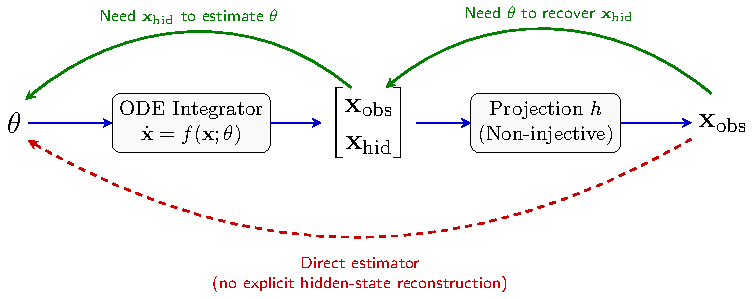
\includegraphics[width=0.8\linewidth]{figures/motive_fig.pdf}
    \caption{Illustration of the forward mapping and the inherent circular dependency in the inverse problem. 
    The forward process generates the full state via an ODE integrator, followed by a non-injective projection $h$ that yields the partial observation $\mathbf{x}_{\text{obs}}$.
    A direct estimator (red dashed arrow) maps the observation to the parameter without forming the hidden state.
    Inverting this process step-by-step requires resolving a circular dependency: estimating the parameter $\theta$ requires the hidden state $\mathbf{x}_{\text{hid}}$ (left green arrow), while recovering $\mathbf{x}_{\text{hid}}$ necessitates prior knowledge of $\theta$ (right green arrow).}
    \label{fig:motive}
\end{figure}

To resolve this dependency, we propose the iterative neural network framework shown in Figure~\ref{fig:method_overview}.
We introduce two neural networks designed to mimic the step-by-step inversion by acting as conditional estimators.
The hidden-state estimator $H_\phi:(\mathbf{x}_\mathrm{obs},\theta)\mapsto \mathbf{x}_\mathrm{hid}$ estimates the hidden state $\mathbf{x}_\mathrm{hid}$ from the observation $\mathbf{x}_\mathrm{obs}$ conditioned on a specific parameter guess $\theta$.
Subsequently, the parameter estimator $P_\psi:(\mathbf{x}_\mathrm{obs}, \mathbf{x}_\mathrm{hid})\mapsto \theta$ refines the parameter guess using the completed trajectory.
These networks are trained independently using decoupled supervised learning to prevent error accumulation, as illustrated in Figure~\ref{fig:method_train}. 
During inference, they are coupled to form a fixed-point iteration operator, continuously updating the parameter estimate as follows:
\begin{equation}
    \hat\theta^{(k+1)}=\mathcal{T}(\hat\theta^{(k)};\mathbf{x}_\mathrm{obs}) := P_\psi(\mathbf{x}_\mathrm{obs},H_\phi(\mathbf{x}_\mathrm{obs},\hat\theta^{(k)})).
\end{equation}
By alternating between the hidden state and parameter updates, the estimate converges to a network-consistent fixed point $\theta^*$ that resolves the circular dependency (whether this network-consistent point is also observation-consistent is the subject of Section~\ref{sec:correctness}).
The remainder of this section details the data representation, the iteration operator $\mathcal{T}$, and the training and inference algorithms.

% figure 위치가 필요한 기호들이 나오기 전에 있어서 약간 이해하기가 곤란한 듯.

\subsection{Data Representation}
\label{subsec:data_gen}

To train the estimators via supervised learning, we generate a synthetic dataset by simulating the dynamics.
We sample parameters $\theta$ and initial conditions $\mathbf{x}(t_0)$ from a predefined training distribution $\mathcal{P}_\mathrm{train}$, solve the initial value problem for the ODE~\eqref{eq:ode} on $[0, T]$ via a numerical solver, and record the states at the sampling times $t_0, \ldots, t_{N}$. 
This procedure yields an i.i.d. dataset $\mathcal{D}$ of $M$ trajectories:

\begin{equation}
\label{eq:training-samples}
\mathcal{D}:=\left\{(\mathbf{x}_{\mathrm{obs}}^{(m)},\mathbf{x}_{\mathrm{hid}}^{(m)},\theta^{(m)})\right\}_{m=1}^M,
\end{equation}
where $\mathbf{x}_{\mathrm{obs}}^{(m)}$ and $\mathbf{x}_{\mathrm{hid}}^{(m)}$ are the flattened vectors defined in Section~\ref{sec:problem}.
Prior to training, these vectors are scaled via a dataset-level normalization scheme (fit on the training split only) to ensure numerical stability.

\subsection{Fixed-Point Iteration Operator}

Given an observation $\mathbf{x}_\mathrm{obs}$, our objective is to accurately infer the corresponding system parameter $\theta$ in accordance with the data generation process as illustrated in Figure~\ref{fig:motive}.
We formulate this parameter estimation as finding a fixed-point of a discrete dynamical system defined by an iterative operator. 
To achieve this, we decompose the estimation problem into two subtasks and construct mappings to perform each.

The first mapping is the hidden-state estimator $H_\phi$, which solves a full state recovery task:
\begin{equation}
    \label{eq:H-map}
        H_\phi:\mathbb{R}^{(N+1)d_{\mathrm{obs}}}\times \mathbb{R}^{p}\to \mathbb{R}^{(N+1)d_{\mathrm{hid}}},
            \quad
        (\mathbf{x}_\mathrm{obs},\theta) \mapsto \hat{\mathbf{x}}_{\mathrm{hid}}.
\end{equation}
This mapping takes the observation $\mathbf{x}_\mathrm{obs}$ and a specific parameter guess $\theta$ as inputs to estimate the corresponding hidden state $\hat{\mathbf{x}}_{\mathrm{hid}}$.
Conditioning on $\theta$ supplies $H_\phi$ with side information that the projection $h$ discards, so that it can estimate a full state trajectory $\mathbf{x}=[\mathbf{x}_\mathrm{obs}, \hat{\mathbf{x}}_\mathrm{hid}]^\top$ consistent with the underlying dynamics; we emphasize that this addresses the non-injectivity of $h$ only relative to the supplied guess, and does not by itself resolve the non-identifiability of $\theta$ from $\mathbf{x}_\mathrm{obs}$ (Section~\ref{sec:correctness}).

The second mapping is the parameter estimator $P_\psi$, which solves a parameter estimation task from the full-state:
\begin{equation}
\label{eq:P-map}
    P_\psi:\mathbb{R}^{(N+1)d_{\mathrm{obs}}}\times \mathbb{R}^{(N+1)d_{\mathrm{hid}}}\to \mathbb{R}^{p},
    \quad
    (\mathbf{x}_\mathrm{obs},\mathbf{x}_{\mathrm{hid}}) \mapsto \hat{\theta}.
\end{equation}
This mapping deduces the parameter vector from the reconstructed full-state trajectory.

We implement both mappings as multi-layer perceptrons (MLPs) parameterized by $\phi$ and $\psi$, respectively; the choice of a flexible, expressive hypothesis class is what makes each conditional mapping learnable from data.

By composing these  two networks, we define the iteration operator $\mathcal{T}(\cdot ;\mathbf{x}_\mathrm{obs}):\Theta \to \Theta$, given by
\begin{equation}
    \label{eqn:iter_oper}
    \mathcal{T}(\theta;  \mathbf{x}_\mathrm{obs}) := P_\psi(\mathbf{x}_\mathrm{obs}, H_\phi(\mathbf{x}_\mathrm{obs}, \theta)).
\end{equation}
This composite operator acts as a discrete dynamical system in parameter space.
We refer to $\mathcal{T}$ as the \emph{fixed-point iteration operator}.
Finding a fixed point $\theta^*$ such that $\theta^*=\mathcal{T}(\theta^*;\mathbf{x}_\mathrm{obs})$ provides a mechanism to resolve the cyclic dependency between two subtasks.

\begin{figure}[htbp]
    \centering
    
    % (a) Training 
    % 가로 배치를 위해 폭을 텍스트 폭의 48%로 설정
    \subfloat[Supervised training via teacher forcing\label{fig:method_train}]{
        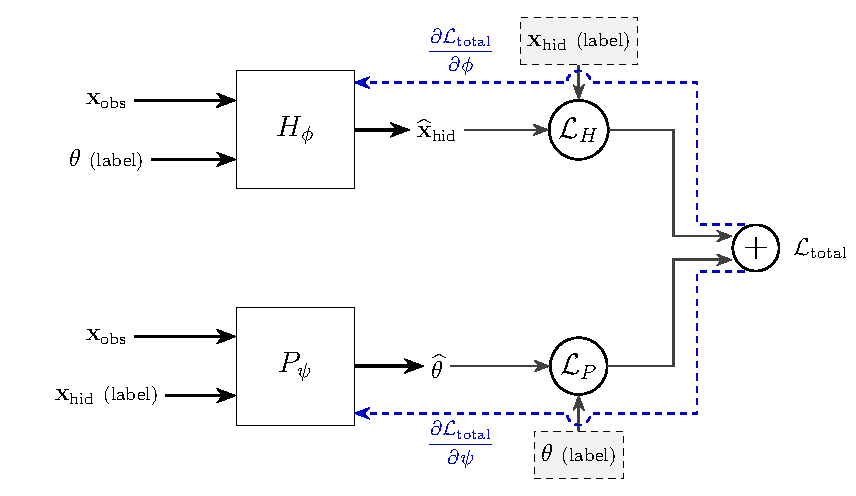
\includegraphics[width=0.50\textwidth]{figures/fig_training.pdf}
    }
    \hfill % 두 그림 사이의 가로 여백
    % (b) Inference
    \subfloat[Inference via alternating iteration\label{fig:method_infer}]{
        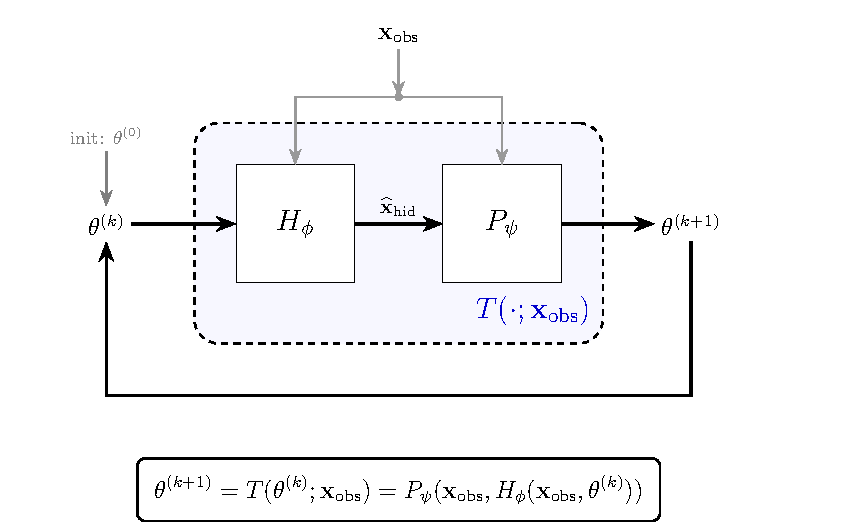
\includegraphics[width=0.45\textwidth]{figures/fig_infer.pdf}
    }
    
    \caption{Overview of the proposed fixed-point iteration networks. 
    The training and inference pipelines are connected but structurally distinct.
    \textbf{(a)} During training, the hidden-state estimator $H_\phi$ and the parameter estimator $P_\psi$ are decoupled. 
    Ground-truth values are provided to optimize $\mathcal{L}_H$ and $\mathcal{L}_P$ independently. 
    \textbf{(b)} At inference, given sparse observations $\mathbf{x}_\mathrm{obs}$, the networks are coupled to define a fixed-point update operator $\mathcal{T}(\cdot; \mathbf{x}_\mathrm{obs})$.}
    \label{fig:method_overview}
\end{figure}

\subsection{Decoupled Supervised Training}
\label{subsec:training}

We train the networks $H_\phi$ and $P_\psi$ in a supervised manner using the synthetic dataset $\mathcal{D}$ generated in Section~\ref{subsec:data_gen}. 
As illustrated in Figure~\ref{fig:method_train}, we train the two networks independently without cyclic dependency to prevent error accumulation. 
This decoupled approach is conceptually analogous to \emph{teacher forcing} \cite{williams1989learning}. 
During inference, $H_\phi$ must rely on a previously estimated parameter $\hat{\theta}^{(k)}$ as its conditional input, and $P_\psi$ must rely on the estimated hidden state $\hat{\mathbf{x}}_{\mathrm{hid}}^{(k+1)}$.
If trained jointly in this coupled manner, early estimation errors would propagate and amplify across the networks.
In our teacher-forced training, we break this cycle by substituting the unavailable inference-phase estimates with exact ground-truth values. 
Specifically, we provide the true parameter $\theta^\mathrm{true}$ as the conditional input to $H_\phi$ (targeting the true $\mathbf{x}_{\mathrm{hid}}^\mathrm{true}$), and provide the true state $\mathbf{x}_{\mathrm{hid}}^\mathrm{true}$ as the conditional input to $P_\psi$ (targeting the true $\theta^\mathrm{true}$).

Given a training sample $(\mathbf{x}_{\mathrm{obs}}, \mathbf{x}_{\mathrm{hid}}^\mathrm{true}, \theta^\mathrm{true}) \sim \mathcal{D}$, we optimize the network parameters $\phi$ and $\psi$ by minimizing their respective mean squared error (MSE) loss functions:
\begin{align}
    \mathcal{L}_H(\phi) &:= \mathbb{E}_{\mathcal{D}} \left[ \left\| H_\phi(\mathbf{x}_{\mathrm{obs}}, \theta^\mathrm{true}) - \mathbf{x}_{\mathrm{hid}}^\mathrm{true} \right\|_2^2 \right], \label{eq:loss_h} \\
    \mathcal{L}_P(\psi) &:= \mathbb{E}_{\mathcal{D}} \left[ \left\| P_\psi(\mathbf{x}_{\mathrm{obs}}, \mathbf{x}_{\mathrm{hid}}^\mathrm{true}) - \theta^\mathrm{true} \right\|_2^2 \right]. \label{eq:loss_p}
\end{align}

Because the two networks do not feed their outputs to one another during training, their computational graphs are strictly disconnected. 
Consequently, when optimizing the total loss $\mathcal{L}_{\mathrm{total}} := \mathcal{L}_H(\phi) + \mathcal{L}_P(\psi)$ via stochastic gradient descent (SGD), the parameter updates are completely decoupled. 
As depicted in Figure~\ref{fig:method_train}, the gradients of the total loss reduce to the partial derivatives with respect to each network's parameters:
\begin{equation}
    \frac{\partial \mathcal{L}_{\mathrm{total}}}{\partial \phi} = \frac{\partial \mathcal{L}_H}{\partial \phi}, \qquad \frac{\partial \mathcal{L}_{\mathrm{total}}}{\partial \psi} = \frac{\partial \mathcal{L}_P}{\partial \psi}.
\end{equation}
These gradients are computed and applied independently without backpropagating errors across the networks. 

This teacher-forced protocol \emph{targets} an operator that preserves the ground truth,
\begin{equation*}
\mathcal{T}(\theta^\mathrm{true}; \mathbf{x}_{\mathrm{obs}}) \approx \theta^\mathrm{true}.
\end{equation*}
Whether the resulting fixed point actually coincides with the ground truth is a separate question, which we take up in Section~\ref{sec:correctness}: there we show that this target is in general unreachable under observational ambiguity, that the fixed point is bounded by the conditional mean, and that under non-identifiability the conditional mean is displaced off the solution fiber.

\subsection{Coupled Inference via Fixed-Point Iteration}
\label{subsec:inference}

Although training is strictly decoupled, inference requires coupling the two networks to form the fixed-point iteration operator $\mathcal{T}$, as illustrated in Figure~\ref{fig:method_infer}. At inference time, only the sparse and partial observation $\mathbf{x}_{\mathrm{obs}}$ is available; the ground-truth parameter and hidden states are completely unknown.

Starting from an initial parameter guess $\hat{\theta}^{(0)}$, we sequentially apply the alternating updates between the hidden-state estimator and the parameter estimator. The overall inference procedure is summarized in Algorithm~\ref{alg:inference}. 

\begin{algorithm}[t]
\caption{Fixed-step iterative inference for parameter estimation}
\label{alg:inference}
\begin{algorithmic}[1]
    \REQUIRE observed samples $\mathbf{x}_\mathrm{obs}=[x_{\mathrm{obs}}(t_0),\ldots,x_{\mathrm{obs}}(t_{N})]^\top$ ($N+1$ times);
    trained networks $H_\phi,P_\psi$; 
    number of iterations $K$
    %\STATE form $\tilde{\mathbf{x}}_{\mathrm{obs}}=\mathrm{vec}(\tilde{x}_{\mathrm{obs},0},\ldots,\tilde{x}_{\mathrm{obs},N-1})$
    %\STATE approximate the derivative features $\widehat{\dot{\mathbf{x}}}_{\mathrm{obs}}$ from $\mathbf{x}_\mathrm{obs}$ via spline interpolation
    %\STATE set $\mathbf{x}_\mathrm{obs}=\left[\mathbf{x}_{\mathrm{obs}},\widehat{\dot{\mathbf{x}}}_{\mathrm{obs}}\right]^\top$
    \STATE initialize $\hat{\theta}^{(0)}$ (e.g., centered at the dataset mean)
    \FOR{$k=0,1,\ldots,K-1$}
        \STATE $\widehat{\mathbf{x}}_{\mathrm{hid}}^{(k+1)} \gets H_\phi(\mathbf{x}_\mathrm{obs},\widehat{\theta}^{(k)})$
        \STATE $\widehat{\theta}^{(k+1)} \gets P_\psi(\mathbf{x}_\mathrm{obs},\widehat{\mathbf{x}}_{\mathrm{hid}}^{(k+1)})$
    \ENDFOR
    \RETURN $\widehat{\theta}^{(K)}$
\end{algorithmic}
\end{algorithm}

The iterative process defined in Algorithm~\ref{alg:inference} is mathematically equivalent to computing the orbit of the discrete dynamical system $\hat{\theta}^{(k+1)} = \mathcal{T}(\hat{\theta}^{(k)}; \mathbf{x}_{\mathrm{obs}})$. For this iteration to be stable and independent of the initial guess, the operator $\mathcal{T}(\cdot; \mathbf{x}_{\mathrm{obs}})$ must be a contraction mapping. We establish sufficient conditions for this contractivity in Section~\ref{sec:convergence}, showing that enforcing appropriate Lipschitz constraints on $H_\phi$ and $P_\psi$ guarantees global geometric convergence to a unique fixed point $\theta^*(\mathbf{x}_{\mathrm{obs}})$. Because of this exponential convergence rate, a very small number of iterations (e.g., $K = 1$ to $10$) typically suffices in practice to reach the fixed point.
